% Chapter 8 of Volume III, "Families, level one from the primes and the step below 7/8". Sources: misc/reviews/nick-volume3/vol3/chG_bondesson.tex lines 1051-1602 (the Code section 1604-1622 cut), referee reports U10 (M1 to M7) and V3A, verification W4 V14. 17 Nov 2026.
\label{bo:ch:families}

Bondesson's oscillator turns the explicit formula into a statement about a function of the cutoff alone (Theorem~\ref{yo:thm:D}). This chapter asks what that instrument can do beyond $\zeta$ and beyond the critical line: for families of $L$ functions, for the level one inequality, which has a proof from the primes, for the Davenport and Heilbronn control, for the step from the half plane $\frac78$ of \cite{OAI26a} to a level just below it, and for $L(s,\chi_{12})$ and $L(s,\Delta)$. Results are from an unrefereed note of Polson (November 2026) unless a source is named. The central order from the explicit formula with the Poisson kernel is in Section~\ref{iw:sec:origin}, and the $\chi_{12}$ kernel in Section~\ref{ch:bpeta} and Section~\ref{sec:ch16:eta}. The oscillator $f$ below is half the oscillator $D$ of Theorem~\ref{yo:thm:D}, so for $\zeta$ its band is $[0,W]$ with $W=4\sum_{\gamma>0}m_\gamma\gamma^{-2}=0.092420$ and its mean is $0.0462$. The half plane $\Re s>\frac78$, in which $\xi$ has no zeros, is the theorem of \cite{OAI26a} (Section~\ref{qrh:sec:claims}). Linear independence of the ordinates (LI) enters only where it is named. Status words follow the book: proved, computed (floating point), conditional with the hypothesis named, heuristic, open.

\section{Ranks from the oscillator and the open questions}\label{bo:sec:oscq}

The gain is in the rate. The classical prime sum integrates the explicit formula once, and we claim no rate for it. The oscillator integrates twice, so each zero enters with weight $\gamma^{-2}$ and under GRH the error is $O(1/\log^2X)$ with an explicit constant (Corollary~\ref{bo:cor:rank}). The ranks of the curves of Remark~\ref{bo:comp:rank} are known unconditionally, by the work of Gross and Zagier~\cite{GrossZagier86} and of Buhler, Gross and Zagier (1985).% TODO for the authors: add the entry Buhler, Gross and Zagier, Math. Comp. 44 (1985), 473 to 481, to the pooled bibliography and cite it here (no key exists). The computation shows that the oscillator is a practical instrument, and that its band is what makes the error explicit.

\paragraph{Open problems.} The state of the oscillator questions is as follows.
\begin{enumerate}
\item Simplicity. Under RH, $\langle f'^2\rangle=\langle f\rangle$ exactly when all zeros are simple (Proposition~\ref{bo:prop:averages}). Open: a version over finite ranges of $L$ with explicit error, which would give a test of simplicity from the primes alone.
\item The walls. Under LI the times near either wall have explicit, extremely small density (Corollary~\ref{bo:cor:walls}). Open: any statement of this kind without LI. Section~\ref{bo:sec:oscwalls} gives one under RH and finitely many checked non relations: density at most $0.05$ for $f<0.01$ and $1.5\times10^{-7}$ for $f<0.001$ (computed). Open: bounds of LI strength without LI.
\item Central zeros. Settled under GRH with explicit error by Corollary~\ref{bo:cor:rank}. Open: an unconditional version. Unconditionally the identity $f=a+bL-P-Q$ holds and if there is a zero with real part $\beta>\frac12$ then $f$ is not $O(e^{cL})$ for any $c<\beta-\frac12$, so the question is whether the parabola can be separated from such growth over a finite range.
\item Families. For a family of $L$ functions, such as quadratic twists, the average of the oscillators is an oscillator for the average explicit formula. Open: the band for the family average, without GRH for the members. This is the family question of Section~\ref{qrh:sec:claims} in the language of this chapter, and it is where the methods behind the quasi Riemann hypothesis might apply. Taken up in Section~\ref{bo:sec:oscfamily}.
\item The band for $\zeta$ itself. Equivalent to RH, and open.
\end{enumerate}

\section{The family problem}\label{bo:sec:oscfamily}

This section takes up the fourth open problem above: what can the oscillator say about a family of $L$ functions that it cannot say about one? There are three findings. The natural family with positive coefficients is a single zeta function in disguise, so it gives a criterion and no new leverage. A family average dilutes an exceptional member, so it cannot see one bad zero. But for the quadratic family the Fej\'er positivity of the oscillator gives, under GRH, a bound on the central order of every member from the primes, which shows nonvanishing at the centre for all but $8$ of the $60786$ fundamental discriminants $|d|\le10^5$ from primes below $3\times10^6$, and recovers heuristically the family proportions of \"Ozl\"uk and Snyder~\cite{OzlukSnyder99}.

\paragraph{The cyclotomic family is one zeta function.} Let $q$ be prime. Summing the oscillators of $L(s,\chi)$ over all characters mod $q$, with $\chi_0$ replaced by $\zeta$, gives the oscillator of the Dedekind zeta function of $\mathbb Q(\zeta_q)$, since $\zeta_{\mathbb Q(\zeta_q)}(s)=\zeta(s)\prod_{\chi\ne\chi_0}L(s,\chi)$. By orthogonality its coefficients $\Lambda(n)\bigl(1+\sum_{\chi\ne\chi_0}\chi(n)\bigr)$ are $(q-1)\Lambda(n)$ for $n\equiv1\bmod q$, $\log q$ at powers of $q$, and $0$ otherwise, so they are nonnegative.

\begin{proposition}[Cyclotomic family]\label{bo:prop:cyclo}
Assume that no $L(s,\chi)$ with $\chi\bmod q$ has a real zero in $(\frac12,1)$. Then the sum over $\chi\bmod q$ of the oscillators satisfies the band criterion of Theorem~\ref{bo:thm:fejer}: it is bounded below for large $L$ if and only if GRH holds for every $L(s,\chi)$ with $\chi\bmod q$.
\end{proposition}

\begin{proof}
The logarithmic derivative of $\zeta_{\mathbb Q(\zeta_q)}$ is a Dirichlet series with nonnegative coefficients, so Landau's theorem applies as for $\zeta$: a singularity on the real axis at the abscissa of convergence. A real singularity to the right of $\frac12$ can only be a real zero in $(\frac12,1)$ (the function $\xi$ has no real zero, and a real character has none at or beyond $1$), and by hypothesis there is none. The poles are at the zeros of all the factors, with positive integer residues, so zeros of different characters cannot cancel, and a nonreal zero of any one factor right of the line forces the sum below every bound.
\end{proof}

So positivity, which is what makes the band a criterion, is bought by summing over the whole character group, and the result, under the hypothesis of the proposition, is the Riemann hypothesis for one larger zeta function. The hypothesis cannot be dropped in this argument: a real zero $\frac12+\delta$ of a real character contributes $2(\cosh(\delta L)-1)/\delta^2>0$ and leaves the sum bounded below, and Landau's theorem then gives only the half plane of that zero. The family is not easier than its members.

\paragraph{Dilution.} If instead the family average has no positivity, it can hide a member. Suppose one member of a family of $M$ has a zero at $\frac12+\delta+i\gamma$. Its contribution to the family average of oscillators is $\frac1M\cdot2\operatorname{Re}\frac{\cosh(zL)-1}{z^2}$ with $z=\delta+i\gamma$, which exceeds the width of the average band only when $e^{\delta L}\gtrsim M|z|^2\overline W$. A family average checked for $L\le L_0$ says nothing about zeros with $\delta<\log M/L_0$. This is the oscillator form of the familiar fact that averages over families give density theorems, not the vanishing of every exceptional zero.

\paragraph{Positivity for each member.} The useful positivity is the one the oscillator already has. For a real primitive character $\chi_d$, $d\ne1$ a fundamental discriminant, of parity $a$, put $g_h(r)=4\sin^2(rh/2)/r^2$, whose Fourier transform is $2\pi(h-|x|)_+$. The explicit formula in Weil's form gives, for every $h>0$,
\[
\frac12\sum_\rho g_h(\gamma_\rho)=f_d(h):=\frac h2\log|d|+G_a(h)-P_d(h),
\]
with $P_d(h)=\sum_{n\le e^h}\chi_d(n)\Lambda(n)n^{-1/2}(h-\log n)$ and $G_a(h)=\frac1{4\pi}\int g_h(r)\bigl(-\log\pi+\operatorname{Re}\psi(\frac14+\frac a2+\frac{ir}2)\bigr)\dd r$. For $\zeta$, with the pole term $16\sinh^2(h/4)$ added, this identity agrees with the sum over the first $6703$ zeros to six digits at $h=2,4,6$ (computed).

\begin{proposition}[Central order from the primes]\label{bo:prop:famrank}
Assume GRH for $L(s,\chi_d)$ and let $m_d$ be the order of its zero at $\frac12$. Then for every $h>0$
\[
m_d\le B_d(h):=\frac{2f_d(h)}{h^2}.
\]
Since $m_d$ is even, $B_d(h)<2$ for one $h$ implies $L(\frac12,\chi_d)\ne0$.
\end{proposition}

\begin{proof}
Under GRH every $\gamma_\rho$ is real, so $g_h(\gamma_\rho)\ge0$, and a central zero contributes $g_h(0)=h^2$. Hence $f_d(h)\ge\frac{m_d}2h^2$. The root number of a real primitive character is $1$, so $m_d$ is even.
\end{proof}

The bound is the oscillator of Theorem~\ref{bo:thm:oscL} evaluated at one point, with its linear term made explicit through the conductor, and it uses only the primes up to $e^h$. The obstruction is visible in the proof: a pair of zeros at height $\gamma$ with $\gamma h$ small contributes almost $h^2$, that is, it imitates a double central zero until $h$ exceeds about $1/\gamma$.

\begin{computation}\label{bo:comp:family}
All $60786$ fundamental discriminants with $|d|\le10^5$, primes to $X=10^5$, $60$ values of $h$; then the remainder with primes to $3\times10^6$ (computed in floating point, under GRH).
% UNVERIFIED: the counts 60731, 47, 8 and the family means are the draft's; U10 checked the arithmetic of the counts only.
\begin{itemize}
\item With primes to $10^5$, $\min_hB_d(h)<2$ for $60731$ discriminants. With primes to $3\times10^6$, $47$ of the remaining $55$ are settled. Under GRH, $L(\frac12,\chi_d)\ne0$ for all but $8$ of the $60786$, the exceptions being $d=-97427$, $-94152$, $-51496$, $-43115$, $-37427$, $-30895$, $-17923$ and $90461$, where the bound stalls between $2.004$ and $2.036$. Nonvanishing at the centre for these conductors is confirmed directly by Platt~\cite{Platt16}, so the computation is a test of the method and not a new fact.
% Platt16 Theorems 7.1 and 7.2: all primitive central values nonzero for conductors up to 2e6 (V3A); resolved.
\item Over $50000<|d|\le10^5$, the family mean of $B_d(h)$ at $h=\log10^5$ is $0.347$. Since $0\le m_d\le B_d$ and $m_d\in\{0,2,4,\dots\}$, under GRH at most $17.4\%$ of these $L(\frac12,\chi_d)$ can vanish, from primes up to the size of the conductor.
\item The family average of $-\Delta_h^2P_d/h^2$, the curvature of Corollary~\ref{bo:cor:rank}, is $-0.30$, $-0.36$, $-0.40$, $-0.43$ at $h=2,3,4,5$, tending to $-\frac12$ with a correction of order $1/h$: it comes from the squares, which are the only $n$ where $\chi_d(n)$ does not average out.
\end{itemize}
\end{computation}

\begin{figure}[ht]
\centering
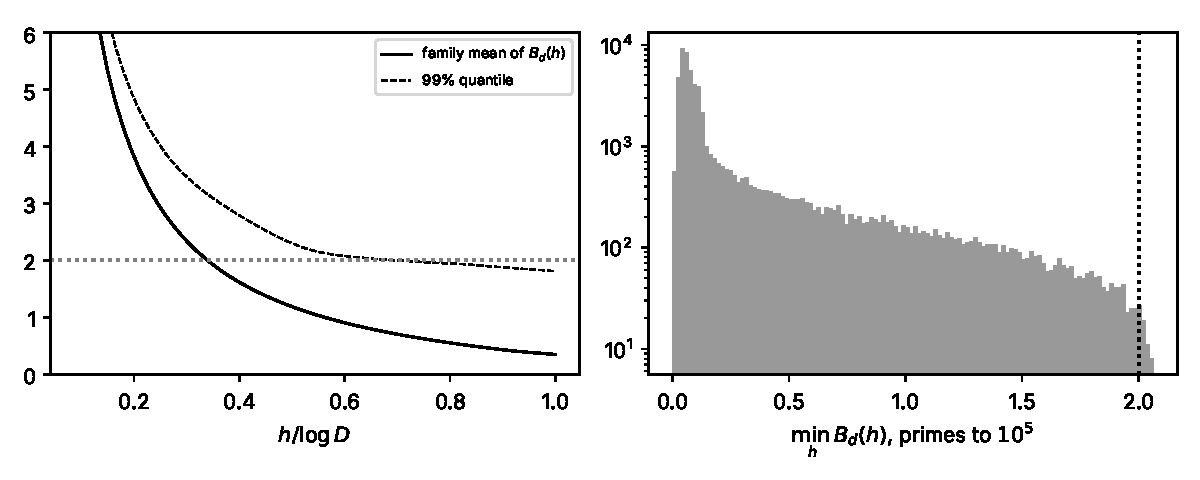
\includegraphics[width=\textwidth]{fig/v3/osc_family.pdf}
\caption{The quadratic family, $|d|\le10^5$, primes to $10^5$. Left: mean and $99\%$ quantile over $50000<|d|\le10^5$ of the bound $B_d(h)$ on the central order, against $h/\log D$; nonvanishing is established below the dotted line. Right: distribution of $\min_hB_d(h)$ over all $60786$ discriminants.}
\label{bo:fig:family}
\end{figure}

\paragraph{The window, and the $-\frac12$.} The last item has a clean reading. Inside the range $e^h<|d|$ the characters $\chi_d(n)$ for $n$ not a square cancel on average over the family, unconditionally by the P\'olya and Vinogradov inequality, and the prime squares give $\overline{P}(h)\approx h^2/4$. In the oscillator this is a parabola of curvature $-\frac12$: on average over the family the members behave as if each had a central zero of order $-\frac12$. This is the oscillator form of the symplectic one level density of Katz and Sarnak~\cite{KatzSarnak99}, whose Fourier transform is $\delta(u)-\frac12$ for $|u|<1$, the zeros of the quadratic family being repelled from the centre. With the family mean of $f_d(h)$ equal to $\frac h2\log D-\frac{h^2}4$ plus lower order terms, the mean bound is $\log D/h-\frac12$, which at the edge of the window $h=\log D$ is $\frac12$, so under this heuristic at least $\frac34$ of the central values are nonzero. If the window extends to $h=2\log D$, where the squares stop growing the mean and the symplectic density predicts no further $-\frac12$, the same computation gives $(\log D)^2/(2h^2)=\frac18$ and a proportion $\frac{15}{16}$. These are the proportions proved under GRH by \"Ozl\"uk and Snyder~\cite{OzlukSnyder99}, who use the same Fej\'er kernel. The window is not proved here, so this paragraph is a heuristic rederivation of known theorems.

\paragraph{Where this leaves the family problem.}
\begin{enumerate}
\item A family band with positivity is a single Riemann hypothesis (Proposition~\ref{bo:prop:cyclo}, under its hypothesis on real zeros); without positivity it is diluted. So family averages cannot by themselves give RH for a member, and the honest target is a density statement.
\item What the family does give, in oscillator form, is the size of the window: the range of $h$, measured against $\log$ of the conductor, over which the off diagonal terms cancel. Unconditionally it is $1$; under GRH it is $2$; Katz and Sarnak predict it is unlimited. Every extension of the window improves the proportion of nonvanishing, and the quasi Riemann hypothesis methods, which beat the diagonal with a mean square over a family of sextic twists, are of exactly this kind.
\item An unconditional version of Proposition~\ref{bo:prop:famrank} is the open problem. Section~\ref{bo:sec:oscuncond} gives it for each $d$ given GRH to a small height, and reduces the family version to one zero statistic. Without GRH, $g_h(\gamma)$ is not positive for complex $\gamma$, and an off line zero contributes $4\sinh^2(\delta h/2)$ type growth with a sign that depends on its height. A density theorem that controls such zeros for $h\le\log D$ on average over the family would give an unconditional positive proportion of nonvanishing in oscillator form; results of this type are known by other methods, through mollified moments, which suggests that the oscillator can be mollified too.
\end{enumerate}

\section{Toward an unconditional version}\label{bo:sec:oscuncond}

Proposition~\ref{bo:prop:famrank} needs GRH only to make each term $\frac12g_h(\gamma_\rho)$ nonnegative. This section measures exactly how much an off line zero can spoil that, and finds three things. Real zeros, including any Siegel zero, cannot spoil it at all. A complex zero at distance $\delta$ from the line costs at most a multiple of $\cosh(\delta h)-1$, which is of second order in $\delta h$. And with GRH verified only to a small height, the bound becomes unconditional: zeros on the line up to height $10$ and the primes below $10^5$ already show $L(\frac12,\chi_d)\ne0$ for $56339$ of the $60786$ discriminants.

\begin{lemma}[Cost of an off line zero]\label{bo:lem:offline}
Let $\rho=\frac12+z$ with $z=\delta+i\gamma$, $|\gamma|>|\delta|$, and put $C=\cosh(\delta h)$. The contribution of $\rho$ to $f_d(h)$ is $(\cosh(zh)-1)/z^2$, and
\[
\operatorname{Re}\frac{\cosh(zh)-1}{z^2}\ \ge\ -\frac{(C-1)(1+\kappa)}{|z|^2},\qquad \kappa=\frac{4\delta^2}{\gamma^2-\delta^2}.
\]
For a real zero, $z=\delta$, the contribution $(\cosh(\delta h)-1)/\delta^2$ is positive.
\end{lemma}

\begin{proof}
With $c=\cos\gamma h$, $s=\sin\gamma h$ and $S=\sinh\delta h$, $\operatorname{Re}\bigl((\cosh(zh)-1)\bar z^2\bigr)=(\gamma^2-\delta^2)(1-Cc)+2\delta\gamma Ss$. Write $1-Cc=-(C-1)+C(1-c)$, and $1-c=2x^2$, $s=2x\cos(\gamma h/2)$ with $x=\sin(\gamma h/2)$. The terms in $x$ form $2(\gamma^2-\delta^2)Cx^2+4\delta\gamma S\cos(\gamma h/2)\,x$, whose minimum over $x$ is at least $-2\delta^2\gamma^2S^2/((\gamma^2-\delta^2)C)\ge-4\delta^2\gamma^2(C-1)/(\gamma^2-\delta^2)$, using $S^2=(C-1)(C+1)$ and $C+1\le2C$. So $\operatorname{Re}\bigl((\cosh(zh)-1)\bar z^2\bigr)\ge-(C-1)\bigl(|z|^2+4\delta^2\gamma^2/(\gamma^2-\delta^2)\bigr)$; divide by $|z|^4$ and use $\gamma^2\le|z|^2$.
\end{proof}

The bound in the lemma is nearly sharp: in a computation, over $\delta\le\frac12$, $1\le\gamma\le400$ and $\frac12\le h\le25$, the minimum of $\operatorname{Re}\frac{\cosh(zh)-1}{z^2}\,|z|^2/(C-1)$ is $-1.06$, against the bound $-(1+\kappa)$.

\begin{theorem}[Unconditional central order bound]\label{bo:thm:uncond}
For every fundamental discriminant $d\ne1$ and every $h>0$,
\[
m_d\ \le\ B_d(h)+\frac{2}{h^2}\sum_{\rho\in\mathcal O_d}\frac{\bigl(\cosh(\delta_\rho h)-1\bigr)(1+\kappa_\rho)}{|\rho-\frac12|^2},
\]
where $\mathcal O_d$ is the set of nonreal zeros of $L(s,\chi_d)$ off the line, assumed to satisfy $|\gamma_\rho|>|\delta_\rho|$ (true if the zeros with $|\gamma|\le\frac12$ are on the line).
If the zeros with $|\gamma|\le T$ are on the line, $T\ge1$, the sum is at most $(\cosh(h/2)-1)\bigl(1+(T^2-\frac14)^{-1}\bigr)S_d(T)$ with $S_d(T)=\sum_{|\gamma|>T}\gamma^{-2}$.
\end{theorem}

\begin{proof}
By the explicit formula $f_d(h)=\sum_\rho(\cosh(zh)-1)/z^2$. Zeros on the line give $2(1-\cos\gamma h)/\gamma^2\ge0$ in pairs and $h^2/2$ at the centre, real zeros give positive terms, and the lemma bounds the rest, under the stated restriction on $\mathcal O_d$. For the second statement use $\delta\le\frac12$ and $|\gamma|>T$.
\end{proof}

The sum $S_d(T)$ is bounded explicitly from the zero counting estimate of Bennett, Martin, O'Bryant and Rechnitzer~\cite{BMOR21}. For a primitive character of conductor $q>1$ and $T\ge\frac57$ with $\ell=\log\frac{q(T+2)}{2\pi}>1.567$, the number $N(T,\chi)$ of zeros with $|\gamma|\le T$ satisfies $|N(T,\chi)-\frac T\pi\log\frac{qT}{2\pi e}+\frac{\chi(-1)}4|\le E(T)$ with $E(T)=0.22737\ell+2\log(1+\ell)-0.5$, and for $\ell\le1.567$ they prove $N(T,\chi)=0$. Partial summation gives $S_d(T)\le\frac{\log(qT/2\pi)+1}{\pi T}+\frac{E(T)}{T^2}+2\int_T^\infty\frac{E(t)}{t^3}\dd t$.

\begin{computation}\label{bo:comp:uncond}
% UNVERIFIED: tables and values of this computation are the draft's, marked computed; W4 and U10 confirmed only the items named in their reports.
With the prime sums of Computation~\ref{bo:comp:family} (primes to $10^5$) and Platt's verification of GRH to height $10^8/q$ for every modulus $q\le4\times10^5$~\cite{Platt16}, Theorem~\ref{bo:thm:uncond} shows $L(\frac12,\chi_d)\ne0$ unconditionally for $60716$ of the $60786$ fundamental discriminants $|d|\le10^5$ (computed in floating point, given that verification). Only $15$ of the discriminants settled under GRH are lost, all of them ones where the GRH bound needed $h$ near $\log10^5$, where $\cosh(h/2)$ is large. The height of verification actually needed is small:
\begin{center}\small
\begin{tabular}{@{}lcccc@{}}
\toprule
zeros on the line up to & $T=3$ & $T=5$ & $T=10$ & $T=20$\\
settled & $15722$ & $44870$ & $56339$ & $59241$\\
\midrule
zeros on the line up to & $T=50$ & $T=100$ & $T=300$ & $T=1000$\\
settled & $60306$ & $60556$ & $60682$ & $60710$\\
\bottomrule
\end{tabular}
\end{center}
\end{computation}

So the oscillator turns the location of the zeros below a modest height, together with a prime sum, into nonvanishing at the centre. For a single $d$ it is quicker to compute $L(\frac12,\chi_d)$ directly, and Platt has done so far beyond this range. The interest is in the mechanism, and in what it says about the family.

\paragraph{The family, without GRH.} Average Theorem~\ref{bo:thm:uncond} over $|d|\le D$ with $h=c\log D$, with $\mathcal O_d$ restricted as in that theorem. Since $m_d\ge0$ is even, the proportion of $d$ with $L(\frac12,\chi_d)=0$ is at most half the mean of $m_d$. With the diagonal evaluation of the mean of $B_d(h)$, $\frac1c-\frac12+o(1)$ for $c\le1$, this gives
\begin{gather*}
\text{proportion of }L(\tfrac12,\chi_d)\ne0\ \ge\ \frac54-\frac1{2c}-\Omega_c(D)-o(1),\\
\Omega_c(D)=\frac1{h^2}\,\mathbb E_d\sum_{\rho\in\mathcal O_d}\frac{(\cosh(\delta_\rho h)-1)(1+\kappa_\rho)}{|\rho-\frac12|^2}.
\end{gather*}
Under GRH $\Omega_c=0$ and $c=1$ gives $\frac34$. Unconditionally the whole question is the size of $\Omega_c$, a family average of off line zeros weighted by $\cosh(c\lambda)-1$, where $\lambda=(\beta-\frac12)\log D$ is the displacement in units of the mean spacing, and by $|\rho-\frac12|^{-2}$, which favours the low zeros. Real zeros do not enter. Any estimate $\Omega_1(D)<\frac34$ gives an unconditional positive proportion, and $\Omega_c<\frac54-\frac1{2c}$ for some $c\in(\frac25,1]$ is enough.

This is a precise target, but an honest look shows it is a strong one. The zero density theorems of Selberg's type~\cite{Selberg46} allow a positive proportion of zeros at displacement $\lambda$ of order one, and those make $\Omega_c$ of order one, not small. What is needed is that the low zeros of the family sit within $o(1/\log D)$ of the line on average, with exponential moments. Positive proportions of nonvanishing for this family are known unconditionally by mollified moments, $\frac78$ in Soundararajan's theorem~\cite{Soundararajan00} for the family $\chi_{8d}$, and the oscillator does not reach that. What the reduction does show is where the difficulty in the oscillator approach lives: not in the primes, whose average is known in the window, and not in Siegel zeros, which are harmless, but in complex zeros a fraction of a mean spacing off the line at low height.

\section{The walls without linear independence}\label{bo:sec:oscwalls}

The wall estimates of Corollary~\ref{bo:cor:walls} assume LI, that the ordinates are linearly independent over $\mathbb Q$, which no computation can verify. This section replaces LI by finitely many statements that a computation can verify: that no integer relation $\sum_jk_j\gamma_j=0$ with small coefficients holds among the first few ordinates. A nonzero real number can be shown nonzero by exact arithmetic, so each such statement is a finite check. The result is a bound, under RH and these checks, on the time the oscillator spends near either wall, down to height $0.01$.

\begin{theorem}[Walls under bounded independence]\label{bo:thm:walls}
Assume RH. Let $\gamma_1<\dots<\gamma_N$ be the first $N$ positive ordinates, $a_j=4/\gamma_j^2$, $\varepsilon>0$, and let $\mathcal R=\{u\in[0,1]^N:\sum_ja_j(1-u_j)\le\varepsilon\}$. Choose integers $M_j\ge0$ and reals $\tau_j\ge0$ (with $0^0=1$), and put
\[
B=\min_{v}\sum_{j}M_j\log\frac{v_j+\tau_j}{1+\tau_j},
\]
the minimum over the vertices $v$ of $\mathcal R$. Suppose there is no relation $\sum_jk_j\gamma_j=0$ with $|k_j|\le M_j$ and $k\ne0$. Then the upper densities in $L$ (logarithmic densities in $Y$) of $\{L:f(L)<\varepsilon\}$ and of $\{L:f(L)>W-\varepsilon\}$, $W=4\sum_{\gamma>0}m_\gamma\gamma^{-2}$, are both at most
\[
e^{-B}\prod_{j=1}^N\mathbb E\Bigl[\Bigl(\frac{U+\tau_j}{1+\tau_j}\Bigr)^{M_j}\Bigr],\qquad \mathbb E[U^i]=\binom{2i}{i}4^{-i},
\]
where $U$ has the arcsine law on $[0,1]$.
\end{theorem}

\begin{proof}
Under RH, $f(L)\ge\sum_{j\le N}a_j(1-u_j)$ with $u_j=\cos^2(\gamma_jL/2)$, all other terms being nonnegative, so $f(L)<\varepsilon$ forces $u(L)\in\mathcal R$. Each $\log\frac{u_j+\tau_j}{1+\tau_j}$ is concave, so $\sum_jM_j\log\frac{u_j+\tau_j}{1+\tau_j}$ attains its minimum over the polytope $\mathcal R$ at a vertex, and is at least $B$ on $\mathcal R$. Hence $\mathbf 1[f<\varepsilon]\le e^{-B}\prod_j\bigl(\frac{u_j+\tau_j}{1+\tau_j}\bigr)^{M_j}$. The right side is a trigonometric polynomial in $L$ with frequencies $\sum_jk_j\gamma_j$, $|k_j|\le M_j$, so its mean exists, and by the hypothesis only $k=0$ survives. That mean factorises, and the mean of a polynomial of degree $M$ in $\cos^2(\theta/2)$ over $\theta$ uniform is its mean under the arcsine law. For the upper wall, $W-f=\sum_\gamma\frac{2m_\gamma}{\gamma^2}(1+\cos\gamma L)$, and the same argument applies with $\sin^2(\gamma_jL/2)$ in place of $u_j$.
\end{proof}

The vertices of $\mathcal R$ are explicit: every coordinate equals $0$ or $1$ except at most one, which takes the value that exhausts the budget $\varepsilon$. For $N\le16$ they can all be listed. The shift $\tau_j$ is what lets an ordinate with $a_j\le\varepsilon$ contribute. For such an ordinate a vertex of $\mathcal R$ can have $u_j=0$, and with $\tau_j=0$ the factor vanishes there and $B=-\infty$. With $\tau_j>0$ it costs only $M_j\log\frac{\tau_j}{1+\tau_j}$ at that vertex.

\begin{computation}\label{bo:comp:walls}
Ordinates to $30$ digits, rounded to integers at scale $10^{14}$ so that all sums are exact, and a meet in the middle search over every coefficient vector in a box; every pair within the rounding radius is rechecked at $30$ digits (computed):
% UNVERIFIED: the relation table and the wall bound table are the draft's; U10 reproduced only the N=4 entry, and W4 did not rerun them.
\begin{center}\small
\begin{tabular}{@{}cll@{}}
\toprule
$N$ & box $(|k_1|,\dots,|k_N|)\le$ & smallest $|\sum k_j\gamma_j|$, $k\ne0$\\
\midrule
$4$ & $(30,20,20,20)$ & $7.6\times10^{-5}$\\
$6$ & $(25,18,15,12,12,10)$ & $3.7\times10^{-6}$\\
$12$ & $(7,6,5,5,4,4,4,3,3,3,3,3)$ & $1.7\times10^{-8}$\\
$14$ & $(8,7,6,5,5,4,4,4,3,3,3,3,3,3)$ & $1.7\times10^{-11}$\\
$16$ & $(8,7,6,5,5,4,4,4,3,3,3,3,3,3,2,2)$ & $3.6\times10^{-13}$\\
\bottomrule
\end{tabular}
\end{center}
The last box has $8.6\times10^{14}$ coefficient vectors; the search took $30$ seconds, and no pair fell within the rounding radius $3.3\times10^{-13}$. So none of these boxes contains a relation. This is a floating point computation with a recheck at $30$ digits. The exclusion of relations is rigorous only if the ordinates carry enclosures of the radius used, which we have not supplied. Optimising $M_j$ and $\tau_j$ in Theorem~\ref{bo:thm:walls}, and checking the majorant on $4\times10^6$ random points of $\mathcal R$, gives under RH alone, for the density of times with $f<\varepsilon$, and equally with $f>W-\varepsilon$:
\begin{center}\small
\begin{tabular}{@{}lccc@{}}
\toprule
$\varepsilon$ & RH and the checks & first version, $\tau=0$ & RH and LI\\
\midrule
$0.01$ & $0.050$ & $1$ & $10^{-23}$\\
$0.007$ & $0.021$ & & \\
$0.005$ & $2.0\times10^{-3}$ & $0.23$ & $10^{-84}$\\
$0.002$ & $5.0\times10^{-6}$ & $1.5\times10^{-3}$ & $10^{-331}$\\
$0.001$ & $1.5\times10^{-7}$ & $2.5\times10^{-6}$ & $10^{-770}$\\
$0.0005$ & $8.7\times10^{-9}$ & $2.3\times10^{-7}$ & $10^{-1511}$\\
$0.0002$ & $2.8\times10^{-9}$ & $1.0\times10^{-7}$ & $10^{-2866}$\\
\bottomrule
\end{tabular}
\end{center}
\end{computation}

Two things improved the bound. The shifts $\tau_j$ bring in ordinates that are individually too high to matter, which is what makes height $0.01$ accessible: the oscillator spends at most $5\%$ of logarithmic time below $0.01$, under RH and checked non relations among $14$ ordinates, against a mean position of $0.046$. The larger boxes, searched exactly, help at small $\varepsilon$, where the bound is limited by the box and not by $\varepsilon$.

The gap to the last column is the price of not knowing LI. Some arithmetic input of this kind is unavoidable. The law of $f$ depends on the relations among the ordinates and not only on their values: if they were all multiples of one number, $f$ would be periodic and would return to $0$, and $\{f<\varepsilon\}$ would have positive density, of order $\varepsilon/\log(1/\varepsilon)$ (of order $\sqrt\varepsilon$ if only finitely many ordinates were involved). A bound smaller than every power of $\varepsilon$, which is what LI gives, needs independence in boxes that grow as $\varepsilon\to0$. The theorem turns that into a computation, and its cost grows like the square root of the number of coefficient vectors.

\section{Where the criterion is a theorem}

\begin{corollary}[A Mertens inequality in Fej\'er form]\label{bo:cor:mertens}
For every $Y>1$, unconditionally,
\[
\sum_{n\le Y}\frac{\Lambda(n)}{n}\Bigl(1-\frac{\log n}{\log Y}\Bigr)\ \le\ \frac{\log Y}{2}+c_1+\frac{1}{\log Y}\sum_{k\ge1}\frac{1-Y^{-(2k+1)}}{(2k+1)^2},
\]
with $c_1=\frac12(\psi(\frac32)-\log\pi)=-0.55412$. The difference of the two sides tends to $\frac{\xi'}{\xi}(1)=c_1+\gamma=0.02310$, where $\gamma$ is Euler's constant. The same holds at every level $\alpha\ge1$.
\end{corollary}

\begin{proof}
At $\alpha=1$ every zero has $\Re(1-\rho)\ge0$, so every term of $S_1(Y)=\sum_\rho\Re\kappa_L(1-\rho)$ is nonnegative, for every $L>0$. The pole block is $\int_0^L(1-w/L)\dd w=L/2$. The limit is part (2) of the proof of Proposition~\ref{bo:prop:margin}, which at $\alpha=1$ needs no hypothesis (a zero on $\Re s=1$ would contribute $\Re(1/(ix))=0$).
\end{proof}

This is the top rung of the ladder in the form of an inequality between elementary quantities, valid for every cutoff and not only for large ones. The proof needs $\Re(1-\rho)\ge0$ only, so it rests on the absence of zeros in the open half plane $\Re s>1$, which is immediate from the Euler product, and by Theorem~\ref{bo:thm:fejer} it is equivalent to that. The nonvanishing on the line $\Re s=1$, and with it the prime number theorem, is not used. The limit of the difference is Li's first coefficient: $c_1+\gamma=1+\frac\gamma2-\frac12\log4\pi=\lambda_1=\sum_\rho\Re\rho^{-1}$.

\begin{computation}\label{bo:comp:mertens}
From the prime powers to $10^7$, on a grid that includes both ends of every interval between consecutive prime powers below $2.7\times10^4$, the difference of the two sides in Corollary~\ref{bo:cor:mertens} is smallest at the largest cutoff, where it is $0.02596$ (computed). It tends to its limit $0.02310$.
\end{computation}

On the critical line itself the inequality follows in a finite range from the verification of the zeros.

\begin{proposition}[Finite range on the line]\label{bo:prop:finite}
Suppose all zeros with $|\gamma|\le H$ are on the critical line. Then for every $Y>1$,
\begin{multline*}
\log Y\cdot S_{1/2}(Y)\ \ge\ 4\sum_{0<\gamma\le H}\frac{\sin^2(\gamma\log Y/2)}{\gamma^2}\\
-\bigl(3+\sqrt Y\bigr)\sum_{\gamma>H}\frac1{\gamma^2}.
\end{multline*}
\end{proposition}

\begin{proof}
Zeros off the line come in quadruples $\frac12\pm d\pm i\gamma$. For the four values $z=\mp d\mp i\gamma$ the terms $1/z$ of $\kappa_L$ cancel in the sum, and the remaining terms are bounded by $(1+e^{-L\Re z})/(L|z|^2)$, which sum to at most $(6+2Y^{d})/(L\gamma^2)$ with $d\le\frac12$. A quadruple has two zeros with $\gamma>0$.
\end{proof}

With $H=3\times10^{12}$, the height of the verification of Platt and Trudgian~\cite{PT21}, the last sum is about $1.5\times10^{-12}$. The first term, computed from the first $6703$ zeros on a grid of step $5\times10^{-4}$ in $\log Y$, is at least $0.0203$ for $1\le\log Y\le47$, and further zeros on the line only increase it (computed: the independent recomputation with $1500$ zeros gives $0.0203$, and the value $0.0209$ of the first computation is not confirmed). For $Y<e$ the oscillator is explicit from the primes: it is positive, tends to $0$ with $\log Y$, and is $0.0160$ at $\log Y=0.01$. Since $(3+\sqrt Y)\times1.5\times10^{-12}<0.0203$ for $Y<1.8\times10^{20}$, the numerical evidence gives $S_{1/2}(Y)>0$ for $1<Y\le10^{20}$. This is a computation and not a proof: the grid carries no bound between its points. A verification to height $H$ establishes the Fej\'er inequality to $Y$ of order $H^2/\log^2H$, and no further: like every finite statement in this volume, it is a corollary of the verification of the zeros.
% UNVERIFIED: 0.0209 (draft) against 0.0203 (W4, 1500 zeros) and the oscillator minimum 0.0205 (draft) against 0.0213 (W4); see U10 M3.

\section{Level one from the primes, and what breaks below it}\label{bo:sec:levelone}

Corollary~\ref{bo:cor:mertens} was proved through the zeros. Since it is equivalent to a fact that needs no zeros, it should have a proof from the primes alone. Finding one shows exactly which properties of the primes the top rung uses, and what would be needed one step down.

\paragraph{The inequality in Mertens form.} Let $r(u)=\sum_{n\le u}\Lambda(n)/n-\log u+\gamma$ be the remainder in Mertens' formula, and $T(Y)=\sum_{n\le Y}\frac{\Lambda(n)}n\log\frac Yn=\int_1^Y\bigl(\sum_{n\le u}\Lambda(n)/n\bigr)\frac{\dd u}u$. Then with $L=\log Y$ and $D_1(L)=\sum_{k\ge1}(1-e^{-(2k+1)L})/(2k+1)^2$,
\[
L\,S_1(Y)=\lambda_1L+D_1(L)-I(Y),\qquad I(Y)=\int_1^Yr(u)\,\frac{\dd u}{u},
\]
so the inequality says that the logarithmic integral of the Mertens remainder satisfies $I(Y)\le\lambda_1L+D_1(L)$, with $\lambda_1=0.0230957$ and $D_1\uparrow\frac{\pi^2}8-1=0.2337$.

\begin{computation}\label{bo:comp:levelone}
% UNVERIFIED: tables and values of this computation are the draft's, marked computed; W4 and U10 confirmed only the items named in their reports.
From the primes to $10^9$ (computed), $I(Y)$ settles at $0.18755$, which is $D_1(\infty)+\sum_\rho(1-\rho)^{-2}=0.23370-0.04615$. The margin $\lambda_1L+D_1(L)-I(Y)$ is $0.077$ at $Y=10^{1/2}$ and increases to $0.525$ at $Y=10^9$; before the first prime, where $I=\gamma L-L^2/2$, it is $0.042$ at $L=0.05$ and larger at the other values checked. For $10^6<u\le10^9$, $|r(u)|\le1.9\times10^{-4}$.
\end{computation}

\begin{theorem}[Level one by elementary means]\label{bo:thm:elementary}
Let $C$ be a constant with $\psi(x)\le Cx$ for all $x\ge1$. Then, using only this bound, the identity $\sum_{d\mid k}\Lambda(d)=\log k$ and the Euler and Maclaurin formula for $\sum_{k\le x}1/k$ and $\sum_{k\le x}\log k/k$,
$S_1(Y)\ge0$ whenever
\[
\lambda_1\log Y\ \ge\ \tfrac12\gamma\log2+\gamma_1+1.0518\,C-\bigl(\tfrac{\pi^2}8-1\bigr)+0.001,
\]
where $\gamma_1=-0.07282$ is the first Stieltjes constant. With $C=\log4$, which is admissible since $\psi(x)<1.04x$ (Rosser and Schoenfeld~\cite{RS62}), this is $\log Y\ge58.6$.
\end{theorem}

\begin{proof}
Let $b=\gamma/\log2=0.8327$ and $w(x)=(1-b)\,1[x\ge1]+b\,1[x\ge2]$, a nonnegative weight. With $H(x)=\sum_{m\le x}1/m$ put
\[
\eta(x)=(1-b)H(x)+b\,H(x/2)-\log x,\qquad x\ge1 .
\]
The choice of $b$ makes $\eta(x)\to0$: for large $x$, $(1-b)(\log x+\gamma)+b(\log x-\log2+\gamma)-\log x=\gamma-b\log2=0$. Now sum $\Lambda(n)/(nm)$ over the pairs with $nm\le Y$, and with $2nm\le Y$, and collect the terms with $nm=k$:
\begin{multline*}
\sum_{n\le Y}\frac{\Lambda(n)}n\Bigl[(1-b)H\Bigl(\frac Yn\Bigr)+b\,H\Bigl(\frac Y{2n}\Bigr)\Bigr]\\
=(1-b)\sum_{k\le Y}\frac{\log k}k+b\sum_{k\le Y/2}\frac{\log k}k=:E(Y).
\end{multline*}
The left side is $T(Y)+\sum_{n\le Y}\frac{\Lambda(n)}n\,\eta(Y/n)$. So
\[
T(Y)=E(Y)-\sum_{n\le Y}\frac{\Lambda(n)}n\,\eta\Bigl(\frac Yn\Bigr).
\]
The first term contains no primes. By the Euler and Maclaurin formula, $\sum_{k\le x}\log k/k\le\frac12\log^2x+\gamma_1+\log x/x$ for $x\ge2$, and we use it only at $x=Y$ and $x=Y/2$ with $\log Y\ge40$, so
\[
E(Y)\le\frac{L^2}2-\gamma L+\tfrac12\gamma\log2+\gamma_1+\frac{2L}{Y}.
\]
For the second term, let $\eta^-=\max(-\eta,0)$ and $G=\sup_{x\ge1}x\,\eta^-(x)$. On $[1,2)$, $\eta(x)=1-b-\log x$, so $x\eta^-(x)$ increases to $2(\log2-1+b)=1.0518$ as $x\to2$. Between consecutive integers $\eta$ is a constant minus $\log x$, so wherever $\eta<0$ the function $x\eta^-(x)$ increases, and its supremum is approached at a left limit $x\to m$, with value $G_m=m\bigl[\log m-(1-b)H_{m-1}-b\,H_{\lfloor(m-1)/2\rfloor}\bigr]$. The Euler and Maclaurin bound $H_{m-1}\ge\log m+\gamma-\frac1{2m}-\frac1{12m^2}$ gives $G_m\le\frac{1+b}2+\frac{1+3b}{12m}\le0.9893$ for even $m\ge4$. For odd $m\ge3$, using also $H_{(m-1)/2}>\log\frac m2+\gamma$, it gives $G_m\le\frac{1-b}2+\frac{1-b}{12m}\le0.0883$. At $m=2$ the value is $2(\log2-1+b)=1.05178\ldots<1.0518$, so $G=2(\log2-1+b)$. Since $\Lambda\ge0$,
\[
-\sum_{n\le Y}\frac{\Lambda(n)}n\,\eta\Bigl(\frac Yn\Bigr)\le\sum_{n\le Y}\frac{\Lambda(n)}n\cdot\frac{G\,n}{Y}=\frac{G\,\psi(Y)}{Y}\le G\,C .
\]
Hence $T(Y)\le\frac12L^2-\gamma L+\frac12\gamma\log2+\gamma_1+GC+2L/Y$. The inequality to be proved is $T(Y)\le\frac12L^2+c_1L+D_1(L)$, and $c_1+\gamma=\lambda_1$; for $L\ge40$ the difference $\frac{\pi^2}8-1-D_1(L)$ and the term $2L/Y$ are together below $0.001$.
\end{proof}

\begin{computation}\label{bo:comp:elementary}
Each step of the proof was checked with the primes to $10^6$. The identity $T=E-\sum\Lambda(n)\eta(Y/n)/n$ holds to all digits ($T(10^6)=87.6472$). $E(Y)-(\frac12L^2-\gamma L)$ decreases to its limit $0.12723$, and is $0.12733$ at $Y=10^5$. The sum $\sum\Lambda(n)\eta(Y/n)/n$ tends to $-0.0603$, and the sum with $\eta^-$ is $0.213$, against the bound $GC=1.458$ used in the proof. The supremum $G=1.0518$ is proved above, and was also confirmed on $[1,400]$. All values in this computation are computed.
\end{computation}

So the top rung has an elementary proof for $Y\ge e^{58.6}$, and it is established by computation for $Y\le10^9$. The gap between is covered by the proof through the zeros.

\begin{computation}[The best step weight]\label{bo:comp:lp}
The proof works for any weight $w(x)=\sum_ja_j1[x\ge d_j]$ with $\sum a_j=1$ and $\sum a_j\log d_j=\gamma$, with the constant $\frac12\sum a_j\log^2d_j+\gamma_1+C\,G_w$ in place of $\frac12\gamma\log2+\gamma_1+1.0518\,C$. Minimising this constant over weights with steps at the integers up to $30$ is a linear programme. A solution of it has steps at $1,\dots,5$ with $a=(0.2194,0.7046,0.0617,0.0089,0.0054)$, $G_w=0.9475$, and constant $1.4628$ against $1.5853$, which lowers the threshold to $\log Y\ge53.3$ (computed). This weight is not optimal: an independent computation in interval arithmetic found an eight step weight with constant below $1.45816$, which lowers the threshold to about $53.1$. We keep $53.3$, the value we reproduced.
\end{computation}

So bounding the error term by its supremum does not close the gap for the weights considered, and we do not expect any weight to.% TODO for the authors (R_bond3 M7): the claim for every weight has a short proof (weighted AM-GM and Jensen give a threshold of at least 32.5, above log 10^9=20.7); add it or keep the softened sentence. The true value of the term is $0.06$, and the supremum bound gives $1.31$ for this weight ($1.458$ for the step weight of Theorem~\ref{bo:thm:elementary}), because it treats the primes in each short range of $n$ as if they could all sit where $\eta^-$ is largest. To do better one needs an upper bound for the number of primes in short intervals, of Brun and Titchmarsh type, which is still free of zeros but is no longer Chebyshev's method. This is a small instance of the lesson of the next paragraphs: each improvement asks for finer information about where the primes are.

\paragraph{What the proof uses.} Three things, which are exactly the three things a proof at any level must find substitutes for.
\begin{enumerate}
\item Positivity of $\Lambda$. It is used once, to replace $-\eta$ by $\eta^-$ and to bound the sum by $\psi(Y)$. This is the Euler product in the form in which the control does not have it.
\item A bound of Chebyshev type, $\psi(Y)\le CY$. It turns the loss into a constant, $GC$.
\item A margin that grows. The inequality has room $\lambda_1L$, linear in $\log Y$, with $\lambda_1>0$. A constant loss is absorbed for large $Y$.
\end{enumerate}

\paragraph{What breaks at level $1-\varepsilon$.} Run the same argument at level $\alpha<1$. The quantity to bound is $T_\alpha(Y)=\sum_{n\le Y}\Lambda(n)n^{-\alpha}\log(Y/n)$, and the convolution identity is now $\sum_{nm=k}\Lambda(n)(nm)^{-\alpha}=k^{-\alpha}\log k$, so the weights are built from $H_\alpha(x)=\sum_{m\le x}m^{-\alpha}=\frac{x^{1-\alpha}}{1-\alpha}+\zeta(\alpha)+O(x^{-\alpha})$. Two of the three ingredients survive and one does not.
\begin{enumerate}
\item Positivity of $\Lambda$ is unchanged.
\item The margin is still linear: by Proposition~\ref{bo:prop:margin} it is $\frac{\xi'}{\xi}(\alpha)\,L$, where the coefficient $\frac{\xi'}{\xi}(\alpha)\approx0.0462(\alpha-\frac12)$ is positive unconditionally, although the statement that the slack tends to it needs the zero location hypothesis of that proposition.
\item The loss is no longer a constant. The remainder of $H_\alpha(x)$ is of size $x^{-\alpha}$, and summed against $\Lambda(n)n^{-\alpha}$ at $x=Y/n$ it gives $Y^{-\alpha}\sum_{n\le Y}\Lambda(n)\,g(Y/n)$ with $g$ bounded. Chebyshev's bound makes this $O(Y^{1-\alpha})$, a power of $Y$, against a margin of size $\log Y$.
\end{enumerate}
So at level $1$ the loss $\psi(Y)/Y$ is bounded and a linear margin absorbs it; at level $1-\varepsilon$ the loss is $Y^{\varepsilon}$ and nothing absorbs it. To repair the argument one needs cancellation in the Chebyshev sum $\sum_{n\le Y}\Lambda(n)g(Y/n)$, where $g$ is a bounded function of mean zero in the logarithmic scale, to the order $Y^{\alpha}\log Y$. That is a power saving in the prime number theorem, which is the statement that there are no zeros to the right of $\alpha$. The elementary method does not fail by a small amount as the level drops below $1$. It fails at once and by a power, because at level $1$ it was using only the size of $\psi$ and below level $1$ it must use the sign changes of $\psi(y)-y$.

\paragraph{The same break, seen as a Tauberian statement.} The criterion at level $\alpha$ reads $\frac1L\int_0^LF_{e^v}(\alpha)\dd v\le c_\alpha+D_\alpha(L)/L$, where $F_Y(\alpha)$ is the sharp truncation of the ledger: the Ces\`aro mean of $F_{e^v}(\alpha)$ in $v$ must stay below the archimedean constant. Its Abel mean is easy at level $1$: $\varepsilon\int_0^\infty F_{e^v}(1)e^{-\varepsilon v}\dd v=F(1+\varepsilon)\to-\gamma$, from the Laurent expansion of $\zeta$ at its pole. Since $F_{e^v}(1)=-\gamma+r(e^v)$ is bounded, by Mertens, Karamata's Tauberian theorem% TODO for the authors: Karamata has no bibliography entry; add one or leave uncited.
 turns the Abel mean into the Ces\`aro mean, and the inequality follows for large $L$ with no reference to zeros at all. At level $\alpha<1$ both steps fail together: the Laplace integral of $F_{e^v}(\alpha)$ converges for every $\sigma>0$ only if there are no zeros to the right of $\alpha$, and the one sided bound that a Tauberian theorem would need is, by Landau's theorem, already equivalent to that. Level $1$ is the last level at which the Dirichlet series itself, and not its continuation, controls the mean.

\section{The control, and the depth of the criterion}

The zero side of Theorem~\ref{bo:thm:fejer} makes sense for any function with a functional equation and a Hadamard product, so the criterion can be calibrated on the control like the other instruments of this volume.

\begin{computation}\label{bo:comp:fejerdh}
% UNVERIFIED: tables and values of this computation are the draft's, marked computed; W4 and U10 confirmed only the items named in their reports.
For the Davenport and Heilbronn function (computed), with its $304$ zeros on the line below height $420$ and its two lowest quadruples, the sum $\sum_\rho\Re\kappa_L(\frac12-\rho)$ is positive for $L<19.57$ and first becomes negative there, at $Y=10^{8.5}$. With the second quadruple alone the first failure is at $L=44.3$, $Y=10^{19.2}$. Both are reproduced to within $2$ per cent by the rule
\[
\log Y^*\approx\frac{\log(0.06\,T^2)}{d}
\]
for a quadruple at height $T$ and distance $d$ from the line.
\end{computation}

The rule comes from comparing the growing term $Y^{d}/(LT^2)$ of the quadruple with the slack $0.0462/L$ of the zeros on the line. It places the Fej\'er criterion among the instruments of Tables~\ref{r:tab:measured} and~\ref{r:tab:distance}. Its depth is logarithmic in the height, which is better than any of the others, and inversely proportional to the distance from the line, like the heat trace. In terms of the number of primes it is costly: the control's first quadruple needs the primes to $3\times10^8$ here. A hypothetical quadruple of $\zeta$ just above the verified range, at height $10^{13}$ and distance $d$, would need $\log Y\approx57/d$.

\paragraph{Summary of the criterion.} Bondesson's method, pushed into the strip, ends in one inequality. Above the line it has a margin linear in the distance to the line. On the line it has none, it has been computed for cutoffs up to $10^{20}$, and its truth for all cutoffs is RH. At level $1$ it is a theorem, a Mertens inequality valid for every cutoff. The slack is at every level the same sum of kernels over the zeros, each nonnegative when its zero lies at or to the left of the level, and on the line, under RH, it is the $2\sin^2$ kernel.

\paragraph{Does this help with a path to RH?} It sharpens the target and does not supply a route. On the side of the target: RH is now one explicit one sided inequality, at one point, between a Fej\'er weighted sum over primes and three closed form terms, and the slack is known exactly under RH: $\log Y\cdot S_{1/2}$ oscillates between about $0.02$ and $0.07$ for $\log Y\ge4$, and on the grids computed it does not approach zero there. The inequality has the right logical shape for route A (Section~\ref{d:sec:A}), since it holds at every level with no zero to the right and fails, by Landau, at every level with one. On the side of the route: the two sides of the inequality are each of size $\sqrt Y/\log Y$ at $\alpha=\frac12$, and the slack is of size $1/\log Y$. To prove the inequality from the primes one must control the Fej\'er mean of $\psi(y)-y$ to relative accuracy $Y^{-1/2}$, which is the strength of RH itself. Nothing in Bondesson's method produces that cancellation; the method names it. The criterion does meet the five requirements of Sections~\ref{route:sec:filters} and~\ref{d:sec:req} as a test: it uses the von Mangoldt function, and it is uniform in height, because it is a statement at the origin for all cutoffs. We have not examined how it behaves along the heat flow.

\section{The size of the arithmetic block, and rigidity}\label{bo:sec:arith}

The last question is how large the $2\sin^2$ transform of the Chebyshev error is at a typical height. Write $A_\alpha(t)=\Re\frac{\zeta'}{\zeta}(\alpha+it)$, so that $J_\alpha(t)=K_\alpha-A_\alpha(t)-P_\alpha(t)$ and the pole term $P_\alpha$ decays. Averaged over $t$, the factor $1-\cos(t\log y)$ is $1$, so $J_\alpha$ has mean $K_\alpha=c_\alpha-\frac{\xi'}{\xi}(\alpha)$, which is negative: $-0.628$ at $\alpha=\frac34$. The arithmetic block is negative on average, and the archimedean block exceeds it by $\frac12\log(t/2\pi)$ on average. For the fluctuation there is a classical mean value: under RH, for fixed $\alpha>\frac12$,
\begin{equation}\label{bo:eq:var}
\lim_{T\to\infty}\frac1T\int_0^TA_\alpha(t)^2\dd t=\frac12\sum_{n\ge2}\frac{\Lambda(n)^2}{n^{2\alpha}},
\end{equation}
which follows from the mean value theorem of Montgomery and Vaughan~\cite{MV74} for Dirichlet polynomials; see Goldston, Gonek and Montgomery (2001).% TODO for the authors: Goldston, Gonek and Montgomery (2001) has no bibliography entry; add it and cite it here. As $\delta\to0$ the right side is $1/(8\delta^2)$ to leading order.

\begin{computation}\label{bo:comp:var}
% UNVERIFIED: tables and values of this computation are the draft's, marked computed; W4 and U10 confirmed only the items named in their reports.
At $6000$ random heights in $[1500,5000]$ (computed), with the density computed from the zeros below $7000$ and a smooth tail:
\begin{center}\small
\begin{tabular}{@{}lcccc@{}}
\toprule
$\alpha$ & $0.60$ & $0.65$ & $0.75$ & $0.875$\\
\midrule
sample variance of $A_\alpha$ & $8.60$ & $4.42$ & $1.71$ & $0.748$\\
prime sum \eqref{bo:eq:var}, all $n$ & $12.09$ & $5.24$ & $1.80$ & $0.755$\\
prime sum, $n\le3000$ & $5.54$ & $3.53$ & $1.61$ & $0.739$\\
independent Cauchy peaks, $\rho\pi/2\delta$ & $15.6$ & $10.4$ & $6.25$ & $4.17$\\
smallest $\pi u_\alpha$ in the sample & $0.289$ & $0.431$ & $0.705$ & $1.02$\\
\bottomrule
\end{tabular}
\end{center}
The sample mean of $A_\alpha$ is below $0.04$ in absolute value. The mean of $\pi u_\alpha$ is $3.06$ to $3.09$.
\end{computation}

Three things follow. First, the variance of the Thorin density about its archimedean trend is a sum over primes, and at the levels $\frac34$ and $\frac78$ the sample agrees with it to $5$ and $1$ per cent; nearer the line the limit \eqref{bo:eq:var} is approached only for $T$ much larger than any $n$ that matters, and the sample lies between the truncated and the full sum. Second, if the zeros were independent points with the same density, the Cauchy peaks would give a variance $\rho\pi/(2\delta)$, which is $1.8$ to $5.6$ times larger than the sample variance. The difference is the rigidity of the zeros, Montgomery's pair correlation~\cite{Montgomery73}, read off the Thorin measure: the primes hold the fluctuation of $U_\alpha$ far below that of a random configuration, and they do so by a formula. Third, away from the origin positivity is never close. At heights $1500$ to $5000$ the smallest value of $\pi u_{3/4}$ among $6000$ samples is $0.705$, against the value $0.0116$ at the origin. The mean is about $2.3$ standard deviations above zero, but the distribution is one sided, a sum of positive peaks, and in the sample it does not come near zero.

\section{Moments of the same measure: the bridge to the chain}

The $2\sin^2$ transform is one transform of the measure $m_\alpha(\dd x)=e^{-\alpha x}\dd R(e^{x})$ on $x=\log y>0$. Its moments are the other, and they are the numbers from which the chain at level $\alpha$ of Chapter~\ref{h:ch:chains} is built.

\begin{proposition}[Prime side power sums]\label{bo:prop:moments}
Let $\alpha>\Theta$ and $k\ge1$. Then
\[
\sum_\rho\frac{1}{(\alpha-\rho)^{k+1}}=\frac{(-1)^k\,\psi^{(k)}(1+\frac\alpha2)}{2^{k+1}\,k!}-\frac1{k!}\int_0^\infty x^k\,m_\alpha(\dd x),
\]
the integral being improper. If the integral is truncated at $x=\log Y$ the error is exactly $\frac1{k!}\int_{\log Y}^\infty x^k\,m_\alpha(\dd x)$, which is $Y^{-\delta}E(Y)(\log Y)^k/k!$ to leading order by Lemma~\ref{bo:lem:trunc}.
\end{proposition}

\begin{proof}
$\frac{\xi'}{\xi}(s)=\frac12\psi(1+\frac s2)-\frac12\log\pi-F(s)$ with $F(s)=\int_0^\infty e^{-sx}\dd R(e^x)$, and $\frac{\xi'}{\xi}(s)=\sum_\rho(s-\rho)^{-1}$. Differentiate $k$ times at $s=\alpha$. The error term comes from Lemma~\ref{bo:lem:trunc} with the extra factor $x^k$.
\end{proof}

\begin{computation}\label{bo:comp:moments}
% UNVERIFIED: tables and values of this computation are the draft's, marked computed; W4 and U10 confirmed only the items named in their reports.
With the primes to $10^9$ (computed): for $k=1$ the prime side gives $-0.0461794$ at $\alpha=1$ against the exact $-0.0461543$, and $-0.046528$ at $\alpha=\frac78$ against $-0.046179$. For $k=2$ and $k=3$ at $\alpha=1$ the errors are $2.6\times10^{-4}$ and $1.9\times10^{-3}$, larger than the quantities themselves, which are $-1.1\times10^{-4}$ and $7.4\times10^{-5}$; they match the error term of the proposition with $E(10^9)\approx0.04$.
\end{computation}

So the square is complete. On the side of the zeros there is the measure $\nu$, whose moments give the chain and whose cosine transform gives the Fej\'er slack. On the side of the primes there is the measure $m_\alpha$, whose moments give the same power sums and whose $2\sin^2$ transform gives the arithmetic block of the Thorin density. The cost is very uneven. The factor $(\log Y)^k/k!\cdot Y^{-\delta}$ is largest at $\log Y=k/\delta$ and decays only beyond it, so the $k$th power sum needs the primes up to about $e^{ck/\delta}$ with $c>1$, while the Taylor coefficients of $\xi$ give it at once. The chain reads the zeros from the kernel cheaply; the primes can supply the same numbers only at a cost exponential in the level.

\section{The distribution over heights: two regimes}

Section~\ref{bo:sec:arith} found the variance of the arithmetic block $A_\alpha(t)$ to be a prime sum. The shape of its distribution is a different matter, and it shows something the variance hides.

\begin{computation}\label{bo:comp:dist}
% UNVERIFIED: tables and values of this computation are the draft's, marked computed; W4 and U10 confirmed only the items named in their reports.
At $20000$ random heights in $[1500,5000]$ (computed), from the zeros:
\begin{center}\footnotesize
\begin{tabular}{@{}lccc@{}}
\toprule
$\alpha$ & $0.60$ & $0.75$ & $0.875$\\
\midrule
skewness of $A_\alpha$, sample & $+1.30$ & $+0.26$ & $-0.04$\\
skewness, random Euler product & $-0.01$ & $-0.09$ & $-0.16$\\
smallest and largest $A_\alpha$ & $-2.96$, $13.4$ & $-2.48$, $5.17$ & $-2.11$, $3.02$\\
share with $A_\alpha<-2$, sample & $0.31$ & $0.033$ & $0.0013$\\
share with $A_\alpha<-2$, model & $0.28$ & $0.069$ & $0.014$\\
share with $A_\alpha<-2.5$, sample & $0.090$ & $0$ & $0$\\
share with $A_\alpha<-2.5$, model & $0.23$ & $0.033$ & $0.0031$\\
share with $A_\alpha<-3$, sample & $0$ & $0$ & $0$\\
share with $A_\alpha<-3$, model & $0.19$ & $0.014$ & $0.0005$\\
\bottomrule
\end{tabular}
\end{center}
The model is the random Euler product, $-\sum_p\log p\,\Re[X_p/(p^{\alpha}-X_p)]$ with independent $X_p$ uniform on the unit circle, sampled $2\times10^5$ times. The Thorin density is negative when $A_\alpha$ is below about $-\frac12\log(t/2\pi)$, which is between $-3.3$ and $-2.7$ on this range.
\end{computation}

The random Euler product is the classical model for $\zeta'/\zeta$ to the right of the critical line, and it gives the correct variance. But at these heights it gives the wrong lower tail. It predicts that the Thorin density at level $\frac34$ would be negative at more than one height in a hundred near $t=3000$, and at level $0.6$ at one height in five. In fact it is negative nowhere, and the sample has no value of $A_\alpha$ below $-3$ at any level. The true distribution is cut off below, and skewed upward by the Cauchy peaks, where the model is nearly symmetric and unbounded.

The reason is that there are two regimes. While the mean spacing of the zeros exceeds $\delta$, that is for $T$ below about $2\pi e^{2\pi/\delta}$, which is $5\times10^{11}$ at $\delta=\frac14$ and $10^{28}$ at $\delta=0.1$, each zero is a separate peak, the density between peaks is a sum of positive tails, and positivity is enforced by the zeros being real and regularly spaced. That is a fact about the functional equation and the rigidity of the zeros, which a model of independent primes does not contain. Beyond that height the peaks overlap, the model becomes appropriate, and its large deviation rate $I(V)$ for the event $A_\alpha<-V$ can be computed from the cumulant generating function of the model. With $V=\frac12\log(T/2\pi)$ the expected number of violations near height $T$ is of order $Te^{-I(V)}$, and
\begin{center}\small
\begin{tabular}{@{}lccccc@{}}
\toprule
$\log_{10}\bigl(Te^{-I}\bigr)$ at $T=$ & $10^6$ & $10^{12}$ & $10^{24}$ & $10^{50}$ & $10^{100}$\\
\midrule
$\alpha=0.60$ & $5.4$ & $9.1$ & $11.4$ & $-8.2$ & $-163$\\
$\alpha=0.75$ & $1.9$ & $-10.1$ & $-137$ & $-1707$ & $-19600$\\
$\alpha=0.875$ & $-5.6$ & $-146$ & $-5400$ & & \\
\bottomrule
\end{tabular}
\end{center}
In each row the model becomes consistent with positivity only at about the height where the peaks begin to overlap, and from there on the expected number of violations falls faster than any power of $T$. This is a heuristic, not a theorem: the model is not justified in the range of large deviations. But the two regimes fit together. At low heights positivity of $U_\alpha$ is a statement about resolved zeros, and at great heights the independence of the primes makes a violation astronomically improbable. Neither regime alone accounts for positivity at all heights, and the transition between them moves to infinity as the level approaches the line.

\section{The step below seven eighths}\label{bo:sec:stepbelow}

The zero free half plane $\Re s>\frac78$ is proved in \cite{OAI26a}; its status, and what it means for the path, are in Section~\ref{qrh:sec:claims}. Does anything in this chapter carry the Thorin property one step down, to the level $\frac78-\varepsilon$? By Theorem~\ref{bo:thm:level} the step is exactly a zero free strip of width $\varepsilon$, and the answer is that the methods here give it for a finite range of cutoffs and no further. The range can be computed, and it shows what the half plane at $\frac78$ buys.

The archimedean part is no obstacle: it moves from $\frac78$ to $\frac78-\varepsilon$ in closed form. The question lives in the criterion of Theorem~\ref{bo:thm:fejer} at the level $\alpha=\theta-\varepsilon$, with $\theta=\frac78$.

\begin{proposition}[Finite range below a zero free level]\label{bo:prop:stepbelow}
Assume $\xi$ has no zeros in $\Re s>\theta$ (for $\theta=\frac78$ this is the theorem of \cite{OAI26a}), and that all zeros with $|\gamma|\le H$ lie on the critical line. Let $\alpha=\theta-\varepsilon>\frac12$ and let $S^{\rm line}_\alpha(Y)$ be the sum of $\Re\kappa_L(\alpha-\rho)$ over the zeros on the line. Then for every $Y>1$,
\[
S_\alpha(Y)\ \ge\ S^{\rm line}_\alpha(Y)-\Bigl[\varepsilon+\frac{Y^{\varepsilon}-1}{\log Y}+\frac{2\varepsilon^2}{H^2\log Y}\Bigr]\sum_{\gamma>H}\frac1{\gamma^2}.
\]
\end{proposition}

\begin{proof}
A zero off the line with $\beta\le\alpha$ contributes a nonnegative term. One with $\alpha<\beta\le\theta$ has $z=\alpha-\rho=-e+ix$ with $0<e\le\varepsilon$ and $|x|>H$. For such $z$, with $R=x^2+e^2$, minimising over the phase gives $\Re\kappa_L(z)\ge-\frac eR-\frac{e^{eL}-1}{LR}-\frac{2e^2}{LR^2}\ge-x^{-2}\bigl[e+\frac{e^{eL}-1}L+\frac{2e^2}{Lx^2}\bigr]$, for every $L>0$. Its partner $1-\bar\rho$ lies to the left of $\alpha$ and contributes a nonnegative term. The zeros with $\beta>\frac12$ and $\gamma>H$ number at most half of all zeros above $H$, and each comes with its conjugate.
\end{proof}

Since $S^{\rm line}_\alpha(Y)$ is close to $\frac{\xi'}{\xi}(\alpha)\approx0.0462(\alpha-\frac12)$ and the sum over $\gamma>H$ is $1.48\times10^{-12}$ at $H=3\times10^{12}$, the criterion at level $\theta-\varepsilon$ is established as long as $Y^{\varepsilon}$ is below about $10^{10}\log Y$.

\begin{computation}\label{bo:comp:stepbelow}
% UNVERIFIED: tables and values of this computation are the draft's, marked computed; W4 and U10 confirmed only the items named in their reports.
The largest $\log Y$ for which Proposition~\ref{bo:prop:stepbelow} gives $S_\alpha(Y)\ge0$, with $H=3\times10^{12}$ and $S^{\rm line}$ computed from the zeros (estimates from the limiting margin and the leading zero counting integral, computed, not enclosures):
\begin{center}\small
\begin{tabular}{@{}lccccc@{}}
\toprule
$\varepsilon$ & $0.2$ & $0.1$ & $0.05$ & $0.02$ & $0.01$\\
level $\frac78-\varepsilon$ & $0.675$ & $0.775$ & $0.825$ & $0.855$ & $0.865$\\
\midrule
(a) granting $\frac78$ & $137$ & $285$ & $588$ & $1523$ & $3120$\\
(b) granting nothing & $83$ & $123$ & $161$ & $196$ & $211$\\
(c) one quadruple & $300$ & $612$ & $1242$ & $3156$ & $6385$\\
\bottomrule
\end{tabular}
\end{center}
Row (a) uses the half plane $\frac78$ of \cite{OAI26a}, that there are no zeros to the right of $\frac78$; its entries are $27$ to $31$ divided by $\varepsilon$. Row (b) grants nothing beyond the verified zeros, and the exponent $\varepsilon$ is replaced by $\frac18+\varepsilon$, the distance from the level to the line $\Re s=1$. Row (c) is the value of $\log Y$ by which a single hypothetical quadruple on the line $\Re s=\frac78$, which the half plane allows, at height $10^{13}$, would make the criterion fail.
\end{computation}

\paragraph{What the hypothesis at seven eighths buys.} It replaces the exponent $\frac18+\varepsilon$ by $\varepsilon$. Without it, the criterion at level $0.865$ is established for $\log Y\le211$. With it, for $\log Y\le3120$. As $\varepsilon\to0$ the established range $\log Y\le30/\varepsilon$ grows without bound, which is the continuity of the criterion in the level. But for each fixed $\varepsilon>0$ it is finite, and beyond it a single quadruple on the line $\Re s=\frac78$, at a height just above the verified range, would break the inequality.

\paragraph{Why the step cannot be taken.} By \cite{OAI26a}, the margin of the criterion at level $\frac78$ is uniform in the cutoff: $S_{7/8}(Y)\ge\frac{\xi'}{\xi}(\frac78)=0.0173$ for every $Y$. For $\log Y\ge0.01$ each zero $\rho$ has $z=\frac78-\rho$ with $0\le\Re z\le\frac34$ and height above $14$, so its kernel term has the right sign, and for $\log Y<0.01$ there are no prime terms and the trivial zeros alone give more than $0.2258$. But the rate at which the criterion changes as the level is lowered is not uniform. A zero at distance $e$ to the right of the level contributes a term that grows like $Y^{e}$, so the derivative in the level grows with $\log Y$, and positivity with room at $\frac78$ passes to $\frac78-\varepsilon$ only for $\log Y$ up to a multiple of $1/\varepsilon$. This is the same break as between level $1$ and level $1-\varepsilon$ in Section~\ref{bo:sec:levelone}: a loss that is a power of $Y$ against a margin that is a multiple of $\log Y$. The half plane at $\frac78$ gives the size of $\psi(y)-y$, namely $O(y^{7/8+\eta})$ for every $\eta>0$, and the step down needs its sign changes.

\paragraph{What does carry over.} Three things, all computational. The density of $U_{7/8-\varepsilon}$ at the origin is positive unconditionally (Proposition~\ref{bo:prop:origin}), and positive for $|t|\le H-\frac12$ where $H$ is the height of the verification. Proposition~\ref{bo:prop:descent} gives an exact test: there are no zeros to the right of $\frac78-\varepsilon$ if and only if $U_{7/8}$ is the Poisson extension by $\varepsilon$ of a positive measure, and the EM descent checks this in a window. And with the archimedean part removed, the descent by $\varepsilon$ is one linear solve (Section~\ref{bo:sec:speed}).

\section{Other $L$ functions: the eta function and the tau function}\label{bo:sec:otherL}

Does the representation help for other $L$ functions? We take the two that are closest to the rest of these books. The Dedekind eta function gives the Dirichlet $L$ function of the even character $\chi_{12}$ modulo $12$, and Ramanujan's function $\Delta$ gives the $L$ function of the tau function:
\begin{align*}
\xi(s,\chi_{12})&=\Bigl(\frac{\pi}{12}\Bigr)^{-s/2}\Gamma\Bigl(\frac s2\Bigr)L(s,\chi_{12})=\int_0^\infty\eta(iy)\,y^{s/2}\,\frac{\dd y}{y},\\
\xi(s,\Delta)&=(2\pi)^{-s}\Gamma(s)L(s,\Delta)=\int_0^\infty\Delta(iy)\,y^{s}\,\frac{\dd y}{y},
\end{align*}
where $\eta(iy)=e^{-\pi y/12}\prod_{n\ge1}(1-e^{-2\pi ny})$ and $\Delta(iy)=\eta(iy)^{24}$.
The first is symmetric about $s=\frac12$ and the second about $s=6$. Both are entire. Four points of the chapter carry over, and each changes in an instructive way.

\paragraph{The archimedean part carries over exactly.} Proposition~\ref{bo:prop:sharp} applies to every gamma factor with real positive shifts. For $\chi_{12}$ the block at level $\alpha$ is $\frac12[\Re\psi(\frac{\alpha+it}2)-\psi(\frac\alpha2)]$, which is $\pi$ times the Thorin density of $g_a(s/4)$ with $a=\frac\alpha2$. For $\Delta$ it is $\Re\psi(\alpha+it)-\psi(\alpha)$, which is $\pi$ times the Thorin density of $g_a$ with $a=\alpha$. An $L$ function of degree $d$ with real positive shifts has $d$ such blocks. The level criterion, Theorem~\ref{bo:thm:level}, holds with the same proof. So Bondesson's letter solves the gamma factor of every $L$ function with real positive shifts. Nonreal shifts produce oscillating factors and need another argument.

\paragraph{There is no pole, and no positive L\'evy measure.} Neither function has a pole, so the divergent negative block of the ledger is absent. But the arithmetic blocks are no longer of one sign: the coefficients of $-L'/L$ are $\chi_{12}(n)\Lambda(n)$, negative on the prime powers with $\chi_{12}=-1$, and $\Lambda_\Delta(p^k)=(\alpha_p^k+\beta_p^k)\log p$ with $\alpha_p+\beta_p=\tau(p)$, negative for $p=2,7,\dots$ So Theorem~\ref{bo:thm:gen} does not apply to the arithmetic factor even to the right of absolute convergence: $L(\alpha+z)/L(\alpha)$ is not the transform of an infinitely divisible law. Bondesson's mechanism, which for $\zeta$ worked down to level $1$, has no range at all here. Positivity of the Thorin measure above the strip is still true, by the level criterion, but it comes from the zeros and not from the signs of the blocks.

\paragraph{The origin is safe, by the product formula.} The kernels $\eta(iy)$ and $\Delta(iy)$ are positive, being infinite products of positive factors. So the completed function is positive on the real axis in both cases, there are no real zeros, and Proposition~\ref{bo:prop:origin} holds with P\'olya's variable replaced by the variable whose density is the kernel in the logarithmic scale. For $\zeta$ the positivity of the kernel was a theorem about a theta series; here it is visible. For a general real character the corresponding kernel need not be positive, and the origin is exactly where an exceptional real zero would enter the ledger: a real zero $\beta>\alpha$ contributes $1/(\alpha-\beta)<0$ to the density at $t=0$. In the language of this section, a Siegel zero is a failure at the origin.

\paragraph{The oscillator has kicks of both signs and no push.} Let $f_\chi$ and $f_\Delta$ be defined as in Theorem~\ref{bo:thm:osc}. The same proof gives
\begin{align*}
f_\chi''(L)&=-\sum_{k\ge0}e^{-(2k+\frac12)L}-\sum_n\frac{\chi_{12}(n)\Lambda(n)}{\sqrt n}\,\delta(L-\log n),\\
f_\Delta''(L)&=-\sum_{k\ge0}e^{-(k+6)L}-\sum_n\frac{\Lambda_\Delta(n)}{n^{6}}\,\delta(L-\log n),
\end{align*}
and, since neither completed function has a real zero, Landau's theorem applies as before: the Riemann hypothesis for the $L$ function holds if and only if $f$ is nonnegative for large $L$, if and only if $f$ is bounded above, and then $0\le f\le4\sum_{\gamma>0}\gamma^{-2}$. The bound is twice the variance of the kernel in the logarithmic scale, which is computed by quadrature.

\begin{computation}\label{bo:comp:otherL}
% UNVERIFIED: tables and values of this computation are the draft's, marked computed; W4 and U10 confirmed only the items named in their reports.
The band widths $4\sum_{\gamma>0}\gamma^{-2}$ (computed) are $0.66585$ for $\chi_{12}$ and $0.22470$ for $\Delta$, from the kernels. With $\tau(n)$ for $n\le4\times10^5$ computed exactly from $\prod(1-q^n)^{24}$, and the primes to the same height, on $0.05\le L\le12.9$:
\begin{center}\small
\begin{tabular}{@{}lcccc@{}}
\toprule
& smallest $f$ & largest $f$ & mean of $f$ & half the band\\
\midrule
$L(s,\chi_{12})$ & $0.1013$ & $0.5418$ & $0.3345$ & $0.3329$\\
$L(s,\Delta)$ & $0.0596$ & $0.1585$ & $0.1126$ & $0.1124$\\
\bottomrule
\end{tabular}
\end{center}
Both oscillators stay inside their bands, and their means agree with the predicted value $2\sum_{\gamma>0}\gamma^{-2}$ to half a per cent and a fifth of a per cent (Figure~\ref{bo:fig:otherL}). No zero of either function was used.
\end{computation}

\begin{figure}[ht]
\centering
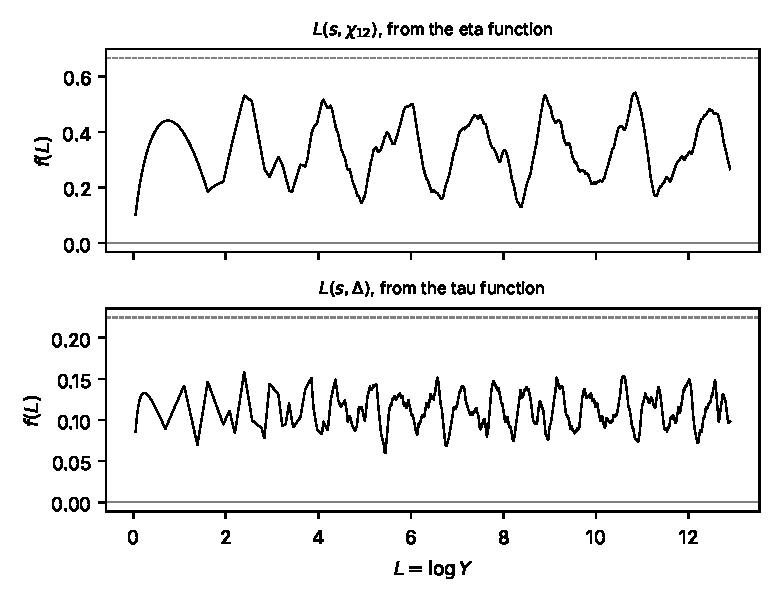
\includegraphics[width=\textwidth]{fig/v3/bo_otherL.pdf}
\caption{The oscillators of $L(s,\chi_{12})$ and $L(s,\Delta)$, computed from the character and from the tau function. Dashed lines are the upper ends of the bands, computed from the kernels $\eta$ and $\Delta$.}
\label{bo:fig:otherL}
\end{figure}

\paragraph{Does it help for these functions?} In the same way as for $\zeta$, and with one gain and one loss. The gamma factor is solved exactly, the level criterion and the descent by deconvolution apply without change, and the criterion at a single point holds with a band that is computable from the kernel. The gain is that there is no pole: the two sides of the criterion are no longer each of size $\sqrt Y$, and the statement is that a Riesz mean of $\chi_{12}(n)\Lambda(n)/\sqrt n$, or of $\Lambda_\Delta(n)/n^6$, differs from a linear function of $\log Y$ by a quantity confined to a fixed band. The loss is that the blocks have both signs, so the one unconditional source of positivity that Bondesson's method had for $\zeta$, a positive L\'evy measure above level $1$, is not available. For these functions the method is purely a ledger. What is special to the two examples is the infinite product, which gives the positivity of the kernel and the absence of real zeros for nothing; the generalised Riemann hypothesis for them is, as for $\zeta$, the statement that the oscillator stays in its band.

\section{What the ledger shows, and whether it helps}

\paragraph{The cancellation is between two divergent Bondesson blocks.} Above level $1$ positivity is a sum of nonnegative blocks minus one finite block, the pole's. In the strip the pole's block is infinite, and the prime blocks must cancel it with an error smaller than the archimedean allowance. Theorem~\ref{bo:thm:ledger} names the difference exactly: it is the $2\sin^2$ transform of the remainder in the prime number theorem. Positivity of the Thorin measure in the strip is a statement about $\psi(y)-y$ seen through Bondesson's kernel.

\paragraph{The margin is linear in the distance from the line, the convergence is a power.} By Proposition~\ref{bo:prop:origin} the room at the binding point is $0.0462\,\delta$, while by Lemma~\ref{bo:lem:trunc} the primes up to $Y$ approach the answer at rate $Y^{-\delta}$, with a constant set by the size of $E$. The cost of seeing positivity at level $\frac12+\delta$ from the primes is therefore about
\[
Y^*(\delta)\approx\Bigl(\frac{13}{\delta}\Bigr)^{1/\delta},
\]
which is $10^{9}$ at $\delta=0.2$, $10^{21}$ at $\delta=0.1$, $10^{48}$ at $\delta=0.05$ and $10^{311}$ at $\delta=0.01$. The descent from the zeros side in the earlier sections costs a noise amplification of only $(T/2\pi)^{\delta/2}$. Positivity in the strip is cheap to see from the zeros and more than exponentially expensive to see from the primes, and the explicit formula is the exchange rate between the two.

\paragraph{The excursions of the prime number theorem are what threaten positivity.} Because only positive excursions of $E$ break \eqref{bo:eq:cert}, the ledger is one sided: the primes running ahead of $y$ is the danger, falling behind is not. Under RH, $E(Y)=O(\log^2Y)$, so \eqref{bo:eq:cert} holds for all large $Y$ at every $\delta>0$. If a zero had real part $\beta>\alpha$, Landau's oscillation theorem would make $R(y)$ exceed $y^{\beta-\varepsilon}$ infinitely often, $E(Y)Y^{-\delta}$ would be unbounded above, and the prime side would fail infinitely often at level $\alpha$, as Theorem~\ref{bo:thm:level} requires.

\paragraph{The origin is the binding point, and the binding term is archimedean.} Every computation of the ledger finds the smallest value of the density, exact or truncated, at $t=0$, where no zero is within $14$ of the point and both Bondesson blocks vanish. With Ces\`aro weights the only negative entry anywhere is the digamma term of the trivial zeros. So the delicate cancellation in the strip is not between primes and zeros at large height, where the zeros are dense and the density is of order $\log t$. It is the low lying one: the gamma factor against the pole and the first few zeros, with a margin $0.0462\,\delta$.

\paragraph{What a proof along this line would need.} Theorem~\ref{bo:thm:cesaro} holds for every $\alpha>\Theta$, so it cannot by itself lower $\Theta$. Read in the other direction it is a criterion: the Ces\`aro truncations are finite sums over primes, and if for some $\alpha$ they were shown to be bounded below by the explicit digamma debt for all large $Y$ and all $t$, the limit would give $U_\alpha\ge0$ and hence, by Theorem~\ref{bo:thm:level}, no zeros to the right of $\alpha$. This is Weil's positivity criterion restricted to the Fej\'er family at level $\alpha$, with the archimedean side written in Bondesson's closed form. It is the precise statement that the $2\sin^2$ transform of the Chebyshev error would have to satisfy.

\paragraph{Why the control fails earlier.} The Davenport and Heilbronn function has no Euler product, so there is no von Mangoldt measure to supply nonnegative blocks, and it has zeros with real part greater than $1$. By Theorem~\ref{bo:thm:level} its Thorin measure already fails above level $1$; there the ledger cannot even be written with a positive arithmetic block. For $\zeta$, Bondesson's blocks are positive because $\Lambda(n)\ge0$, which is the Euler product, and that is the one place the Euler product requirement of Section~\ref{route:sec:filters} enters the ledger.

\paragraph{Does it help?}

For computation, yes. The letter solves the gamma factor exactly, at every level. It does not make iterative deconvolution converge faster, but it makes a single linear solve accurate, which is ten thousand times cheaper than EM (Section~\ref{bo:sec:speed}). It turns the descent from a known positive level, such as $1$ or $\frac78$ (the latter by \cite{OAI26a}), into the deconvolution of a remainder with mean zero. That improves linear deconvolution by one to two orders of magnitude. It also pins down the drift that the arithmetic part must cover near $t=0$, and it gives an explicit GGC reference law $g_a$ for Monte Carlo inversion.

For proof inside the strip, no. By Theorem~\ref{bo:thm:level}, positivity at a level below one is equivalent to a zero free half plane, and Bondesson's mechanism stops where infinite divisibility stops, at $\alpha=1$. Proposition~\ref{bo:prop:descent} describes exactly what a proof would have to show starting from the theorem of \cite{OAI26a} at $\frac78$. The present numerics verify it only in a window.

\section{Open problems}

\begin{enumerate}
\item Factorisation in the strip. Find smoothed Dirichlet polynomials or approximate functional equation models of $(s-1)\zeta(s)$ whose reciprocals at level $\alpha$ are GGC transforms up to a drift that fits inside the archimedean budget $\frac12\log(t/2\pi)$ on windows $[T,2T]$.
\item Let $\alpha_P$ be the least level at which the truncated Euler product times the archimedean factor is a GGC transform. Is it true that $\alpha_P\to1$? Compute $\alpha_P$ for $P\le10^4$.
\item Detection bounds. For EM descent from $\frac78$ with grid step $h$ and $K$ iterations, find the smallest detectable $\varepsilon$ as a function of $h$, $K$ and the local gap. Run the test near the Lehmer pairs.
\item Accelerate the EM with Nesterov momentum and test it at heights $10^4$ to $10^6$ using zeros from Odlyzko's tables~\cite{OdlyzkoTables}, applied to the detrended remainder.
\item Prove that the integral in Lemma~\ref{bo:lem:trunc} is $o(Y^{-\delta})$ on average, so that \eqref{bo:eq:cert} is an exact criterion in the limit, and prove that under RH the Ces\`aro truncated density of Theorem~\ref{bo:thm:cesaro} is positive for all $t$ once it is positive at the origin, as Computation~\ref{bo:comp:cesaro} finds on $[0,60]$.
\item By Proposition~\ref{bo:prop:margin} the slack returns arbitrarily close to zero, and by Computation~\ref{bo:comp:records} the smallest grid value up to $L=2\times10^5$ is $0.01795$. Prove a lower bound for $f(L)$ in terms of $L$ under RH, from the theory of simultaneous approximation.
\item Characterise the kick trains for which the oscillator of Theorem~\ref{bo:thm:osc} stays in a band. Random kicks do not and the control's do not (Computations~\ref{bo:comp:random} and~\ref{bo:comp:controlosc}). Is there a model with fluctuating zeros, such as a function built from finitely many Euler factors or a random matrix model with a functional equation, in which boundedness can be proved?
\item Theorem~\ref{bo:thm:elementary} and Computation~\ref{bo:comp:lp} prove the level one inequality by elementary means for $\log Y\ge58.6$, and for $\log Y\ge53.3$ with the weight of Computation~\ref{bo:comp:lp}. Close the gap down to the computed range, using the Brun and Titchmarsh inequality for the error term, to give a proof for every $Y>1$ that uses no zeros.
\item At level $1-\varepsilon$ the elementary argument needs $\sum_{n\le Y}\Lambda(n)g(Y/n)=O(Y^{1-\varepsilon}\log Y)$ for one explicit bounded $g$. Is there any $\varepsilon>0$ and any family of weights for which this follows from a sieve or a mean value estimate?
\item Find the order $n^*$ at which the Pick test on $G_\alpha^{(n+1)}/G_\alpha^{(n)}$ first fails, by analogy with Remark 4$'$ of Bondesson's letter, and how $n^*$ depends on $\alpha$.
\end{enumerate}
